\chapter{Transformaciones}
\label{cha:Transformaciones}

Una vez detallados todos los aspectos fundamentales relacionados con la caracterización de antenas, estamos a disposición de profundizar en nuestro objeto de estudio principal. El cual abordaremos siguiendo un camino natural que pasa por presentar y entender transformaciones sencillas que nos proporciones una base solida que nos permita dar el salto a la transformación de campo cercano a campo lejano en coordenadas esféricas.

\section{Definición del campo cercano y lejano}

Aunque en la introducción hablábamos de los términos de campo cercano y campo lejano, no dimos una definición formal de qué significaban, por lo que vamos a dedicar esta sección precisamente a esto. Una forma simple de entender el por qué se diferencia entre campo cercano y lejano consiste en estudiar el comportamiento de una onda conforme se aleja de la fuente que la provocó. Si estudiamos el comportamiento de una onda electromagnética, veríamos que conforme se aleja de la fuente que la generó más se asemeja a un frente de ondas plano hasta que llega a un punto donde directamente podemos aproximar que la onda tiene el mismo comportamiento que una onda plana.

\begin{figure}[h]
    \centering
    \includegraphics[scale=0.60]{Figura7-Esquema para ejemplificar el paso de onda esferica a onda plana}
    \caption{Representación visual del paso de onda esférica a onda plana}
    \label{Ejemplo-paso-onda-esferica-a-onda-plana}
\end{figure}

Precisamente es este punto en el cual la onda puede considerarse como onda plana donde se define la frontera entre campo cercano y campo lejano. De forma que los valores del campo donde aún no podemos aproximar que la onda tiene un comportamiento plano pertenecen al campo cercano, mientras que aquellos valores donde la onda se aproxima a una onda plana pertenecen al campo lejano.\\ 

En términos exactos, el campo lejano se define como la región en la que el frente de onda saliente de una antena es plano y la variación del patrón de radiación es independiente con respecto a la distancia de la propia antena. Por lo tanto, para considerar una onda perteneciente al campo lejano, su componente radial debe ser despreciable en comparación con la componente transversal y la relación entre el campo eléctrico y magnético debe ser igual a la impedancia intrínseca del medio. Debiéndose cumplir ambos requisitos en todas las direcciones angulares vistas desde la antena.
\\

Esto supone que para determinar la distancia a partir de la cual tenemos medidas pertenecientes al campo lejano hay que verificar estas propiedades para todas las direcciones angulares, cosa que ocurre a una distancia igual a:

\begin{equation}
                            R =\frac{2D^2}{\lambda}
\end{equation}

\noindent
donde D es la dimensión máxima de la antena y $\lambda$ es la longitud de onda de operación.\\

Si recordamos, esta fórmula ya la habíamos presentado al detallar las limitaciones presentes al usar una cámara anecoica. Lo que ilustra que, en realidad, todo el rato hemos tratado con la idea de campo lejano y campo cercano.
\newpage

\section{Transformación entre puntos del campo cercano}

La primera transformación que vamos a abordar para adquirir una base sólida de cara a afrontar las siguientes secciones consiste en transformar un punto de un plano $Z_1$ cualquiera perteneciente a la región de campo cercano a otro plano $Z_2$ perteneciente también a la región de campo cercano.

% Representaci ́on de los planos Z1 y Z_2 en perspectiva isometrica
\tdplotsetmaincoords{60}{125} % Establecer la perspectiva
\begin{figure}[htbp]
  \centering
  \begin{tikzpicture}[tdplot_main_coords,scale=2]
    % Plano Z1 en azul
    \fill[blue!20] (0,0,0) -- (2,0,0) -- (2,2,0) -- (0,2,0) -- cycle;
    \draw[blue] (0,0,0) -- (2,0,0) -- (2,2,0) -- (0,2,0) -- cycle;
    \node[blue] at (1,1,0) {\( Z_1 \)};
    % Plano Z2 en rojo
    \fill[red!20] (0,0,1) -- (2,0,1) -- (2,2,1) -- (0,2,1) -- cycle;
    \draw[red] (0,0,1) -- (2,0,1) -- (2,2,1) -- (0,2,1) -- cycle;
    \node[red] at (1,1,1) {\( Z_2 \)};
    % Ejes
    \draw[thick,->] (0,0,0) -- (2.5,0,0) node[anchor=north east]{\( x \)};
    \draw[thick,->] (0,0,0) -- (0,2.5,0) node[anchor=north west]{\( y \)};
    \draw[thick,->] (0,0,0) -- (0,0,1.5) node[anchor=south]{\( z \)};
  \end{tikzpicture}
  \caption{Representación de los planos \( Z_1 \) y \( Z_2 \) en perspectiva isométrica.}
  \label{fig:planos_NF_Z1_Z_2}
\end{figure}

Para ello, nos a basaremos en el manual de C.Balanis \autocite{Balanis_2016} para hacer un desarrollo previo que nos permita introducir de forma ordenada las ecuaciones fundamentales que debemos utilizar.
\\

Lo primero que debemos hacer es definir la expresión de un campo eléctrico genérico y de frecuencia $\omega$.

\begin{equation}
\vec{\tilde{E}}(\vec{r},t)=\vec{E}(\vec{r})\,e^{j\omega t}
\label{NFtoNF: eq-Campo E generico}
\end{equation}

Tras esto, debemos recordar la ecuación de onda del campo eléctrico, la cual tiene la siguiente forma:

\begin{equation}
\nabla^{2} \vec{\tilde{E}}(\vec{r},t)=\frac{1}{c}\frac{\partial^{2}
\vec{\tilde{E}}(\vec{r},t)}{\partial t^{2}}
\label{NFtoNF: eq-de-onde-campo-electrico}
\end{equation}

\noindent
donde $c$ representa la velocidad de propagación de la onda.\\

Desde esta expresión, podemos llegar a la ecuación de Helmholtz basándonos en \autocite{Pozar}.

\begin{equation}
(\nabla^{2}+k^{2})\vec{E}(\vec{r})=0
\label{NFtoNF: eq-Helmholtz}
\end{equation}

\noindent
con $k=\frac{\omega}{c}$

\newpage

Si ahora consideramos el campo $\vec{\tilde{E}}(\vec{r})$ como uno sobre el que podemos tomar medidas pertenecientes a un plano paralelo al eje $XY$ situado a una altura $z=z_{m}$ análogo a los planos vistos en la figura \ref{fig:planos_NF_Z1_Z_2}, entonces la función bidimensional $\vec{E}(x,y,z=z_{m})$ se puede representar
mediante una integral de Fourier de la siguiente forma:

\begin{equation}
\vec{E}(x,y,z=z_{m})=\int_{-\infty}^{\infty}\int_{-\infty}^{\infty}\vec{\hat{E}}(k_{x},k_{y},z=z_{m})
\,e^{-j (k_{x} x+k_{y} y)} dk_{x} dk_{y}
\label{NFtoNF: eq-fourier-campo-electrico}
\end{equation}

\noindent
expresión que podemos introducir en \eqref{NFtoNF: eq-Helmholtz}, obteniendo:

\begin{multline}
\left(\nabla^{2}+k^{2}\right)\left(\int_{-\infty}^{\infty}\int_{-\infty}^{\infty}\vec{\hat{E}}(k_{x},k_{y},z)
\,e^{-j (k_{x} x+k_{y} y)} dk_{x}
dk_{y}\right)=\\
\int_{-\infty}^{\infty}\int_{-\infty}^{\infty}\left(\nabla^{2}+k^{2}\right)\left[\vec{\hat{E}}(k_{x},k_{y},z)
\,e^{-j (k_{x} x+k_{y} y)}\right] dk_{x} dk_{y}=0
\label{NFtoNF: eq-fourier-campo-electrico-introducida-en-Helmholtz}
\end{multline}

\noindent
donde hemos devuelto la generalidad a la componente $z$ debido a que a efecto de los cálculos puede tomar cualquier valor. Hasta ahora era específica para reforzar la relación de esta componente con los planos de medida.
\\

Si ahora operamos el Laplaciano, obtenemos:

\begin{equation}
\int_{-\infty}^{\infty}\int_{-\infty}^{\infty}\left[\left(-k_{x}^{2}-k_{y}^{2}+k^{2}\right)+\frac{\partial^{2}}{\partial
z^{2}}\right]\left[\vec{\hat{E}}(k_{x},k_{y},z) \,e^{-j (k_{x}
x+k_{y} y)}\right] dk_{x} dk_{y}=0.
\label{NFtoNF: eq-fourier-campo-electrico-introducida-en-Helmholtz-con-laplaciano-operado}
\end{equation}

\noindent
como esta igualdad debe cumplirse para todos los valores de $x$ e $y$, el integrando ha de ser nulo. Lo que da como resultado:

\begin{equation}
\frac{\partial^{2}}{\partial
z^{2}}\vec{\hat{E}}(k_{x},k_{y},z)+w^{2}\vec{\hat{E}}(k_{x},k_{y},z)=0
\label{NFtoNF: resultado eq-fourier-campo-electrico-introducida-en-Helmholtz simplificada}
\end{equation}

\noindent
donde $w^{2}=k^{2}-k_{x}^{2}-k_{y}^{2}$.\\

A partir de esta expresión, podemos definir una solución general de \eqref{NFtoNF: resultado eq-fourier-campo-electrico-introducida-en-Helmholtz simplificada} de la siguiente forma:

\begin{equation}
\vec{\hat{E}}(k_{x},k_{y},z)=\vec{\mathcal{E}^{+}}(k_{x},k_{y})\,e^{-j
w z}+\vec{\mathcal{E}^{-}}(k_{x},k_{y})\,e^{j w z}
\label{NFtoNF: solucion eq-fourier-campo-electrico-en-Helmholtz-general}
\end{equation}

\noindent
donde el valor $\vec{\mathcal{E}^{+}}(k_{x},k_{y})\,e^{-j w z}$  representa una onda propagada en el sentido positivo del eje $z$, mientras que, como contrapartida, $\vec{\mathcal{E}^{-}}(k_{x},k_{y})\,e^{j w z}$ representa una onda propagada en dirección opuesta.\\


Para nuestro caso, solamente consideraremos la solución que contiene la onda $\vec{\mathcal{E}^{+}}(k_{x},k_{y})\,e^{-j w z}$, por lo que podemos reescribir la ecuación \eqref{NFtoNF: eq-fourier-campo-electrico} teniendo en cuenta solo esta solución. Obteniendo el mísmo resultado que el visto en la ecuación (12-73) en \autocite{Balanis_2016}.

\begin{equation}
\vec{E}(x,y,z)=\int_{-\infty}^{\infty}\int_{-\infty}^{\infty}\vec{\mathcal{E}^{+}}(k_{x},k_{y})
\,e^{-j (k_{x} x+k_{y} y+w  z)} dk_{x} dk_{y}
\label{NFtoNF:eq-fourier-balanis}
\end{equation}

\newpage

\subsection{Algoritmo para transformar el valor del campo cercano medido en $z=z_{1}$ en el campo cercano en otro plano $z=z_{2}$}
\label{sec:Algoritmo NFtoNF}


Partiendo del desarrollo hecho en la sección anterior, estamos a disposición de generar un algoritmo que nos permitirá calcular el campo eléctrico en una posición $z$ cualquiera que no tiene por qué ser la de salida de la onda. Es decir, no tiene por qué corresponderse con el plano radiante de la antena en el que hemos obtenido las medidas, sino que puede ser cualquier plano posterior. Esto significa que hablamos de un algoritmo capaz de calcular el campo cercano en un plano geométrico dado por una $z$ concreta a partir de los valores del campo medido en un plano anterior cualquiera independientemente de si este plano pertenece a la región de campo cercano o lejano. Esto es debido a que todo lo anterior es válido independientemente del valor de  $z$ a partir del cual consideramos que nuestro campo pasa a ser lejano.
\\

Lo primero que debemos hacer es estimar los modos dados por la función
$\vec{\hat{E}}(k_{x},k_{y},z=z_{1})$, para lo cual, hay que partir de la
ecuación \eqref{NFtoNF: eq-fourier-campo-electrico} e invertirla \footnote{En realidad, \eqref{NFtoNF:eq-fourier-campo-electrico-invertida} tiene la forma de
la transformada de Fourier directa de $\vec{E}(x,y,z=z_{1})$ como
función de $x$ e $y$, mientras que la ecuación \eqref{NFtoNF: eq-fourier-campo-electrico}
es formalmente la transformada inversa}, lo que nos da la siguiente ecuación:

\begin{equation}
\vec{\hat{E}}(k_{x},k_{y},z=z_{1})=\frac{1}{(2\pi)^{2}}\int_{-\infty}^{\infty}\int_{-\infty}^{\infty}\vec{E}(x,y,z=z_{1})
\,e^{j (k_{x} x+k_{y} y)} dx dy.
\label{NFtoNF:eq-fourier-campo-electrico-invertida}
\end{equation}

\noindent
No obstante, debido a que las medidas de las que partimos no son continuas, sino que conocemos el campo $\vec{E}(x,y,z=z_{1})$ en un conjunto de puntos
$(x,y)=(x_{n_{x}},y_{n_{y}})$ con $n_{x}=0,1,2,\ldots,N_{x}-1$ y
$n_{y}=0,1,2,\ldots,N_{y}-1$, deberemos discretizar nuestro problema teniendo en cuenta que en lugar de un plano continuo como el mostrado en la figura \ref{fig:planos_NF_Z1_Z_2} tendremos lo siguiente: 

\begin{figure}[h]
    \centering
    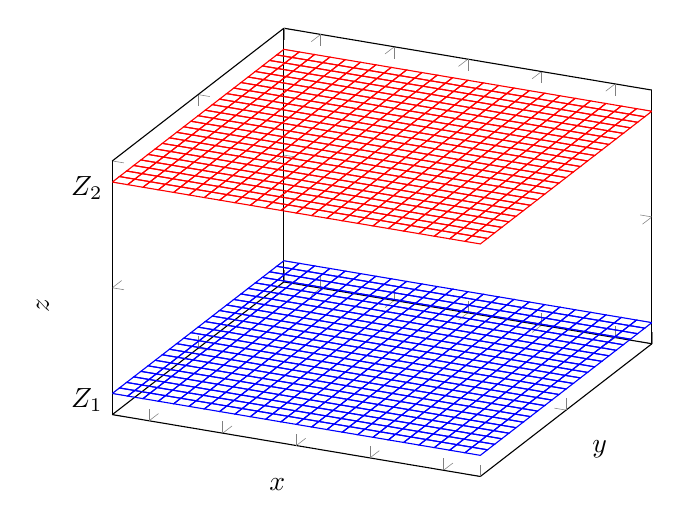
\begin{tikzpicture}[scale=1]
        \begin{axis}[
            xticklabels={,,},
            yticklabels={,,},
            zticklabels={$Z_{2}$, ,$Z_{1}$, ,$Z_{2}$},
            zlabel=$z$,
            xlabel=$x$,
            ylabel=$y$
            ]
            \addplot3[mesh] {5};
            \addplot3[mesh] {7};
        \end{axis}
    \end{tikzpicture}
    \caption{Representación de los planos $Z_{2}$ y $Z_{1}$ de forma discreta.}
    \label{fig:planos_NF_Z1_Z_2_discretos}
\end{figure}

\noindent
Debido a esto, deberemos discretizar \eqref{NFtoNF: eq-fourier-campo-electrico} y, por tanto,  \eqref{NFtoNF:eq-fourier-campo-electrico-invertida}, por lo que vamos a reescribirla de la siguiente forma:

\begin{equation}
\vec{\hat{E}}(k_{x},k_{y},z=z_{1})=\frac{\Delta x
\Delta y}{(2\pi)^{2}}
\sum_{n_{x}=0}^{N_{x}-1}\sum_{n_{y}=0}^{N_{y}-1}\vec{E}(x=n_{x}\Delta
x,y=n_{y} \Delta y,z=z_{1}) \,e^{j (k_{x} n_{x} \Delta x+k_{y} n_{y}
\Delta y)}
\label{NFtoNF:eq-fourier-campo-electrico-invertida-discretizada}
\end{equation}

\newpage

A partir de \eqref{NFtoNF:eq-fourier-campo-electrico-invertida-discretizada} se pueden obtener las componentes modales para cualquier valor de $(k_{x},k_{y})$. Con ellas se puede reconstruir el campo completo empleando la fórmula \eqref{NFtoNF: eq-fourier-campo-electrico}. De forma que, aparentemente, nos interesaría utilizar el mallado más fino posible en términos de $(k_{x},k_{y})$ para que la integral de \eqref{NFtoNF: eq-fourier-campo-electrico}, al aproximarse por su versión de sumatorio discreto, se calcule con el menor error posible. La malla original de los datos del campo eléctrico tiene una densidad de $N_{x} x N_{y}$ que condiciona la resolución real alcanzable en nuestra estimación.\\

Sin embargo, necesitamos tener en cuenta lo siguiente:
\begin{enumerate}
    \item No estamos teniendo en cuenta el teorema del muestreo dado que no por
    tomar más valores de $(k_{x},k_{y})$ vamos a tener una mejor descripción
    de $\vec{E}(x,y,z)$, sino que en realidad hay un nivel de información máximo
    asociado al muestreado en $(x,y)$.
    
    \item Afrontar el problema de esta forma no nos permite vincularlo con el algoritmo de la transformada rápida de Fourier (FFT), lo que nos impide beneficiarnos de las características fundamentales de este algoritmo.

\end{enumerate}

\noindent
Debido a esto, tenemos un especial interés en poder resolver nuestro problema con el algoritmo de la FFT ya que tanto la FFT como su inversa (IFFT) son algoritmos que tienen esto en cuenta. Llegados a este punto es interesante estudiar brevemente ambas expresiones, por lo que vamos a comenzar definiendo la expresión de la FFT. 

\begin{equation}
\vec{\hat{E}}_{m_{x},m_{y}}=\frac{1}{N_{x} N_{y}}
\sum_{n_{x}=0}^{N_{x}-1}\sum_{n_{y}=0}^{N_{y}-1}
\vec{E}(x=n_{x}\Delta x,y=n_{y} \Delta y,z=z_{1}) \,e^{j 2\pi
\frac{m_{x} n_{x}}{N_{x}}}\,e^{j 2\pi \frac{m_{y} n_{y}}{N_{y}}}
\label{NFtoNF:eq-fft1}
\end{equation}

\noindent
y a continuación la expresión de la IFFT.

\begin{equation}
\vec{E}_{n_{x},n_{y}}=
\sum_{n_{x}=0}^{N_{x}-1}\sum_{n_{y}=0}^{N_{y}-1}
\vec{\hat{E}}_{m_{x},m_{y}} \,e^{-j 2\pi \frac{m_{x}
n_{x}}{N_{x}}}\,e^{-j 2\pi \frac{m_{y} n_{y}}{N_{y}}}
\label{NFtoNF:eq-ifft1}
\end{equation}

Si compararamos  \eqref{NFtoNF:eq-fft1} con \eqref{NFtoNF:eq-ifft1}, vemos que para
poder aprovechar la herramienta que nos brinda la FFT debemos cumplir las siguientes igualdades:

\begin{subequations}
\begin{align}
k_{x}&= m_{x}\Delta k_{x}
\\
k_{y}&= m_{y}\Delta k_{y}
\\
\Delta x \Delta k_{x}&=\frac{2\pi}{N_{x}}
\\
\Delta y \Delta k_{y}&=\frac{2\pi}{N_{y}}.
\end{align}
\end{subequations}

\newpage

De todas ellas, las más relevantes para nosotros son las dos últimas debido a que son de obligado cumplimiento si queremos poder interpretar la ecuación \eqref{NFtoNF:eq-fourier-campo-electrico-invertida-discretizada} como
una FFT. Pudiendo definir\footnote{Si nos fijamos, $\Delta x$ y $\Delta y$ están
definidos por el muestreado del campo medido en $z_1$. Pero los de $\Delta k_{x}$ y $\Delta k_{y}$ aún no estaban definidos.} los valores de $\Delta k_{x}$ y
$\Delta k_{y}$ como:

\begin{align}
\Delta k_{x}&=\frac{2\pi}{\Delta x N_{x}}
\\
\Delta k_{y}&=\frac{2\pi}{\Delta y N_{y}}
\end{align}

Teniendo esto en cuenta, podemos definir la relación entre 
$\vec{\hat{E}}_{m_{x},m_{y}}$ de la ecuación \eqref{NFtoNF:eq-fft1} y 
$\vec{\hat{E}}(k_{x},k_{y},z=z_{1})$ de la ecuación \eqref{NFtoNF:eq-fourier-campo-electrico-invertida-discretizada} como:

\begin{equation}
\vec{\hat{E}}(k_{x}=m_{x} \Delta k_{x},k_{y}=m_{y} \Delta
k_{y},z=z_{1})= \Delta x \Delta y\vec{\hat{E}}_{m_{x},m_{y}}
\end{equation}

Expresión que, a nivel computacional, usaremos para calcular los modos $\vec{\hat{E}}(k_{x}=m_{x} \Delta k_{x},k_{y}=m_{y} \Delta
k_{y},z=z_{1})$ de la siguiente forma:

\begin{equation}
\vec{\hat{E}}_{m_{x},m_{y}}=\mbox{FFT}\{\vec{E}(x=n_{x}\Delta
x,y=n_{y} \Delta y,z=z_{1})\}.
\label{NFtoNF:eq-FFT-del-campo}
\end{equation}

Llegados a este punto, entramos en la segunda parte del proceso de transformación, donde haremos uso de la IFFT como herramienta para poder calcular el campo en $z=z_2$, para lo cual debemos discretizar \eqref{NFtoNF:eq-fourier-balanis} para poder aproximarnos a \eqref{NFtoNF:eq-ifft1} de la siguiente forma:

\begin{equation}
\vec{E}(x,y,z=z_{2}) =
\\
\Delta k_{x} \Delta k_{y}
\sum_{m_{x}=0}^{N_{x}-1}\sum_{m_{y}=0}^{N_{y}-1} 
\vec{\hat{E}}(k_{x},k_{y},z=z_{2})
\,e^{-j(n_{x}m_{x}\Delta x  \Delta k_{x} + n_{y}m_{y}\Delta xy  \Delta k_{y})}
\end{equation}

Haciendo uso de la ecuación \eqref{NFtoNF: solucion eq-fourier-campo-electrico-en-Helmholtz-general} y manteniendo que $\vec{\mathcal{E}^{-}}(k_{x},k_{y})=0$, entonces se cumple que:

\begin{equation}
\vec{\hat{E}}(k_{x},k_{y},z_{1})=\vec{\mathcal{E}^{+}}(k_{x},k_{y})\,e^{-j
w z_{1}}
\end{equation}

\noindent
expresión a partir de la cual podemos despejar $\vec{\mathcal{E}^{+}}(k_{x},k_{y})$ como:

\begin{equation}
\vec{\mathcal{E}^{+}}(k_{x},k_{y})=\vec{\hat{E}}(k_{x},k_{y},z_{1})\,e^{j
w z_{1}}
\label{NFtoNF:Ez2-cambio-fase}
\end{equation}

Lo que finalmente nos permite calcular el campo en $z=z_2$ como:

\begin{equation}
\vec{E}(x,y,z=z_{2})=\Delta k_{x} \Delta
k_{y}\,\mbox{IFFT}\{\vec{\hat{E}}(k_{x}=m_{x}\Delta
k_{x},k_{y}=m_{y} \Delta k_{y},z=z_{2})\}.
\label{NFtoNF:Ez2-final}
\end{equation}

\newpage

Finalmente, Conviene matizar las siguientes observaciones:
\begin{enumerate}
    \item Como el campo es vectorial, hay que aplicar separadamente este
    algoritmo a todas las componentes.
    \item Podemos trabajar con $\Delta x=\Delta y$.
    \item Los dos planos y las dos rejillas de medidas tienen que tener las mismas
    dimensiones pero pueden ser subdominios de áreas mayores en las
    cuales, por lo que sea, eliminamos ciertos márgenes. Eso ocurre en
    el caso de trabajar con medidas simuladas sobre espacios esféricos,
    donde los cortes con $z$'s dados no son iguales: nos quedamos con
    los subdominios de iguales dimensiones.
\end{enumerate}

\newpage
\subsection{Validación del algoritmo}

Una vez detallado el proceso teórico necesario para transformar las medidas del campo cercano, estamos a disposición de demostrar con un ejemplo que nuestra transformación es válida.\\
Para ello, vamos a realizar una simulación en COMSOL de una antena microstrip de la cual extraeremos los valores del campo cercano medido sobre un plano $Z_1$ que usaremos para calcular el campo cercano en un plano posterior $Z_2$.
\\

La antena microstrip que hemos construido en la simulación presenta las siguientes características básicas:

\begin{itemize}
    \item Tiene un punto de alimentación de $50\Omega$.
    \item La frecuencia de trabajo sera de 1.575 Ghz.
    \item Las dimensiones W y L de la antena son 7 mm y 15.5 mm.
\end{itemize}

\begin{figure}[h]
    \centering
    \includegraphics[scale=0.65]{Simulaciones COMSOL/MS-Planta de la antena}
    \caption{Esquemático de la antena microstrip en COMSOL.}
    \label{Simulaciones COMSOL/MS-Planta de la antena}
\end{figure}

\noindent

Correspondiéndole el siguiente diagrama de radiación:

\begin{figure}[h]
  \centering
    \includegraphics[scale=0.65]{Simulaciones COMSOL/MS-Diagrama de radiación}
    \caption{Diagrama de radiación de la antena simulada.}
    \label{MS-Diagrama de radiación de la antena simulada}
\end{figure}

\newpage

Una vez hecha la simulación, hemos desarrollado un programa en Python que implementa lo visto en \ref{sec:Algoritmo NFtoNF} utilizando los datos extraídos de la antena microstrip. No obstante, lo primero que debemos verificar es que estamos leyendo correctamente los datos extraídos de COMSOL, lo cual podemos hacer si enfrentamos la representación del campo a una distancia $Z_1$ devuelta por COMSOL con la obtenida en nuestro programa tras leer los datos.\\

En nuestro caso, vamos a tomar las medidas del campo medido sobre el plano $Z_1=15mm$ y las usaremos para obtener el campo en el plano $Z_2=30mm$, por lo que vamos a utilizar el módulo del campo en el plano $Z_1$ para la comprobación, que en la simulación tiene la siguiente forma:

\begin{figure}[h] 
  \centering
    \includegraphics[scale=0.5]{Simulaciones COMSOL/MS-Enorm a 15mm}
    \caption{Módulo del campo medido en $Z_1=15mm$ en COMSOL.}
    \label{MS-Diagrama de radiación de la antena simulada}
\end{figure}

\newpage

Mientras que este mismo corte representamos desde nuestro programa a partir de los datos ledos de la simulación tiene la siguiente forma:

\begin{figure}[h] 
  \centering
    \includegraphics[scale=0.8]{Resultados python/MS-Enorm a 15mm python}
    \caption{Módulo del campo medido en $Z_1$ reconstruido en python.}
    \label{MS-Diagrama de radiación de la antena simulada}
\end{figure}

Como vemos, ambas representaciones coinciden, lo que confirma que tanto el programa como la simulación trabajan con los mismos datos, por lo que podemos realizar los cálculos que nos permiten calcular el campo en el plano posterior $Z_2$ y enfrentarlos a la simulación. Cabe destacar que el propósito de esta sección es únicamente demostrar que la transformación genera valores correctos. Debido a esto, nos vamos a centrar únicamente en los resultados y dejar la explicación del programa para el anexo correspondiente.\\

El primero de los resultados que vamos a estudiar es la representación bidimensional de la FFT de las componentes cartesianas del campo. 

\begin{figure}[h]
    \centering
    \begin{tikzpicture}
        % Inserta la imagen original
        \node[anchor=south west,inner sep=0] (image) at (0,0) {\includegraphics[scale=0.70]{Resultados python/MS-FFT 2D Ex a 15mm python.png}};

        % Dibuja un rectángulo en la esquina superior izquierda
        \begin{scope}[x={(image.south east)},y={(image.north west)}]
            \draw[red,thick] (0.1,0.7) rectangle (0.3,0.9); % Cambia los valores para ajustar la posición y tamaño del rectángulo
        \end{scope}
        
         % Inserta la imagen aumentada usando coordenadas específicas
        \node[anchor=south west] (zoomed) at (-4.5,0.4) {\includegraphics[scale=0.40]{Resultados python/MS-FFT 2D Ex a 15mm python ZOOM.png}};
        
                % Flecha roja
        \begin{scope}[x={(image.south east)},y={(image.north west)}]
            \draw[thick,->,red] (0.1,0.7) -- (-0.08,0.588);
        \end{scope}
        
    \end{tikzpicture}
    
    \caption{FFT 2D de la componente $E_x$ del campo en $Z_1$}
    \label{FFT 2D Ex a 15mm}
\end{figure}

\begin{figure}[h]
    \centering
    \begin{tikzpicture}
        % Inserta la imagen original
        \node[anchor=south west,inner sep=0] (image) at (0,0) {\includegraphics[scale=0.70]{Resultados python/MS-FFT 2D Ey a 15mm python.png}};

        % Dibuja un rectángulo en la esquina superior izquierda
        \begin{scope}[x={(image.south east)},y={(image.north west)}]
            \draw[red,thick] (0.1,0.7) rectangle (0.3,0.9); % Cambia los valores para ajustar la posición y tamaño del rectángulo
        \end{scope}
        
         % Inserta la imagen aumentada usando coordenadas específicas
        \node[anchor=south west] (zoomed) at (-4.5,0.4) {\includegraphics[scale=0.40]{Resultados python/MS-FFT 2D Ey a 15mm python ZOOM.png}};
        
                % Flecha roja
        \begin{scope}[x={(image.south east)},y={(image.north west)}]
            \draw[thick,->,red] (0.1,0.7) -- (-0.08,0.588);
        \end{scope}
        
    \end{tikzpicture}
    
    \caption{FFT 2D de la componente $E_y$ del campo en $Z_1$}
    \label{FFT 2D Ey a 15mm}
\end{figure}

\newpage

\begin{figure}[h]
    \centering
    \begin{tikzpicture}
        % Inserta la imagen original
        \node[anchor=south west,inner sep=0] (image) at (0,0) {\includegraphics[scale=0.70]{Resultados python/MS-FFT 2D Ez a 15mm python.png}};

        % Dibuja un rectángulo en la esquina superior izquierda
        \begin{scope}[x={(image.south east)},y={(image.north west)}]
            \draw[red,thick] (0.1,0.7) rectangle (0.3,0.9); % Cambia los valores para ajustar la posición y tamaño del rectángulo
        \end{scope}
        
         % Inserta la imagen aumentada usando coordenadas específicas
        \node[anchor=south west] (zoomed) at (-4.5,0.4) {\includegraphics[scale=0.40]{Resultados python/MS-FFT 2D Ez a 15mm python ZOOM.png}};
        
                % Flecha roja
        \begin{scope}[x={(image.south east)},y={(image.north west)}]
            \draw[thick,->,red] (0.1,0.7) -- (-0.08,0.588);
        \end{scope}
        
    \end{tikzpicture}
    
    \caption{FFT 2D de la componente $E_z$ del campo en $Z_1$}
    \label{FFT 2D Ez a 15mm}
\end{figure}

Estas figuras corresponden al resultado de la ecuación \eqref{NFtoNF:eq-FFT-del-campo} y en ellas se muestran cuatro componentes modales situadas en las esquinas. 

\newpage

Partiendo de los resultados anteriores, debemos aplicar la IFFT tras haber aplicado previamente el cambio de fase tal y como veíamos en \eqref{NFtoNF:Ez2-final} y \eqref{NFtoNF:Ez2-cambio-fase}, lo que nos devuelve los siguientes resultados:

\begin{figure}[h] 
  \centering
    \includegraphics[scale=0.70]{Resultados python/MS-IFFT 2D Ex a 15mm python}
    \caption{IFFT 2D de la componente $E_x$ del campo en $Z_1$}
    \label{IFFT 2D Ex a 15mm}
\end{figure}

\begin{figure}[h] 
  \centering
    \includegraphics[scale=0.70]{Resultados python/MS-IFFT 2D Ey a 15mm python}
    \caption{IFFT 2D de la componente $E_y$ del campo en $Z_1$}
    \label{IFFT 2D Ex a 15mm}
\end{figure}
\newpage
\begin{figure}[h] 
  \centering
    \includegraphics[scale=0.70]{Resultados python/MS-IFFT 2D Ez a 15mm python}
    \caption{IFFT 2D de la componente $E_z$ del campo en $Z_1$}
    \label{IFFT 2D Ex a 15mm}
\end{figure}

\newpage

A partir de los resultados de la IFFT podemos calcular finalmente el campo en el plano $Z_2=30mm$. Obtenido que su módulo en $Z_2$ tiene la siguiente forma:

\begin{figure}[h] 
  \centering
    \includegraphics[scale=0.70]{Resultados python/MS-Enorm a 30mm python}
    \caption{Módulo del campo eléctrico en el plano $Z_2$}
    \label{IFFT 2D Ex a 15mm}
\end{figure}

De nuevo, para verificar que este resultado es válido vamos a enfrentar esta representación del modulo con la obtenida en la simulación de COMSOL. La cual tiene la siguiente forma:

\begin{figure}[h] 
  \centering
    \includegraphics[scale=0.40]{Simulaciones COMSOL/MS-Enorm a 30mm}
    \caption{Módulo del campo medido en $Z_2$ en COMSOL.}
    \label{IFFT 2D Ex a 15mm}
\end{figure}

Si nos fijamos, las representaciones coinciden pero los valores máximos difieren ligeramente. Esto se debe a que la escala de COMSOL sitúa los colores rojos a partir de 6 $V/m$ y la librería de Python usada para representar el módulo los situa a partir de 7 $V/m$

\newpage

Una forma adicional de verificar los resultados pasa por restar los valores del módulo reconstruidos y simulados puesto que independientemente de la escala de color, la resta debería dar un campo prácticamente nulo como vemos que ocurre en la siguiente figura: 

\begin{figure}[h] 
  \centering
    \includegraphics[scale=0.70]{Resultados python/MS-Enorm comparación cuantitativa python}
    \caption{Comparación cuantitativa del campo simulado y calculado.}
    \label{IFFT 2D Ex a 15mm}
\end{figure}

En la figura \ref{IFFT 2D Ex a 15mm} podemos ver cómo la resta de los valores pertenecientes al campo se anulan dejando una región circular central a cero mientras que los valores externos a la circunferencia presentan patrones residuales que no tienen relación con el campo surgidos de los cálculos.

\newpage

\section{Transformación del campo cercano medido en una superficie plana a campo lejano en coordenadas esféricas}
\label{sec:validación NFtoNF esférico}
% //Esto es una demostración de lo visto en el punto anterior. NO es una transformación.

Una vez comprendido el proceso teórico que nos permite transformar medidas entre dos planos medidos en campo cercano y tras haber validado que transformación es correcta, debemos verificar que podemos obtener las medidas del campo cercano efectuadas sobre un plano en coordenadas cartesianas y calcular con ellas las medidas pertenecientes en una superficie esférica.\\

Lo primero que haremos será partir de la definición de un campo eléctrico cualquiera cuyos valores pertenecen al campo lejano.

\begin{equation}
\vec{E}(x,y,z)=\frac{jk_{z}}{2\pi r}\,e^{-jk_{0}r}{\vec{\mathcal{E}}}(k_{x}=k \sin\theta \cos\phi,k_{y}= k\sin\theta \sin\phi)
\label{NFtoFF:eq-campo-lejano}
\end{equation}

\noindent
donde $k_{x}$ y $ k_{y}$  contienen la información de los ángulos del sistema de referencia esférico que sirve de base para la expresión del diagrama de radiación en el campo lejano y  $k_{z}=k\cos\theta$. Siendo $k$ el número de onda en el vacío.\\

Para nuestra transformación, lo que realmente nos interesa es el valor del espectro, es decir, la función de modos ${\vec{\mathcal{E}}}(k_{x},k_{y})$. La cual responde a la siguiente expresión:

\begin{equation}
{\vec{\mathcal{E}}}(k_{x},k_{y})=\int_{-\infty}^{\infty}\int_{-\infty}^{\infty}\vec{E}(x,y,z=z_{0})\,e^{-j k_{x}x}\,e^{-jk_{y}y} dx dy.
\label{NFtoFF:eq-modos-del-campo-lejano}
\end{equation}
 
En la ecuación \eqref{NFtoFF:eq-modos-del-campo-lejano} podemos extraer una característica muy importante,  que la extracción de las componentes modales no depende del plano $z$, sino que puede tomar cualquier valor. Lo que significa que, mientras las medidas de dicho plano pertenezcan al campo cercano, la descomposición será siempre la misma.\\
Por otro lado, debemos tener en cuenta que en realidad solo conoceremos como es el campo  $\vec{E}(x,y,z=z_{0})$ en un conjunto discreto de puntos $(x,y) = (x_{n_{x}},y_{n_{y}})$ con  $n_{x}=0,1,2,\ldots,N_{x}-1$ y  $n_{y}=0,1,2,\ldots,N_{y}-1$. Debiendo reescribir nuestra ecuación de modos para que se ajuste a este conjunto de valores a la vez que adaptamos la ecuación para que podamos hacer uso de la transformada discreta de Fourier para poder hacer uso de la FFT.

Tras este razonamiento, vamos a reescribir la ecuación \eqref{NFtoFF:eq-modos-del-campo-lejano} de la siguiente forma: 
\begin{align}
{\vec{\mathcal{E}}}(k_{x},k_{y})&=\frac{L_{x}L_{y}N_{x}N_{y}}{4 \pi^2 (N_{x}-1)(N_{y}-1)} \nonumber \\
&\times \sum_{n_{x}=1}^{N_{x}-1}\sum_{n_{y}=1}^{N_{y}-1} DFT(\vec{E}(x=n_{x}\Delta
x,y=n_{y}\Delta
y,z=z_{0}))\,e^{-j k_{x}n_{x} \Delta x}\,e^{-jk_{y}n_{y} \Delta y}
\label{NFtoFF:eq-fourier}
\end{align}
\noindent
donde:

\begin{itemize}
    \item $N_{x}$ y $N_{y}$ son respectivamente el número de puntos del campo cercano en la dirección $x$ e $y$ .
    \item $L_{x}$ y $L_{y}$  es la longitud de la apertura en las dimensiones  $x$ e $y$.
\end{itemize}

\newpage

\noindent
De esta forma, la ecuación \eqref{NFtoFF:eq-fourier} corresponde a la descomposición modal del campo. Sin embargo, debemos discretizando los valores de $k_{x}$ y $k_{y}$ para poder aplicar la DFT aplicando las siguientes expresiones: 

\begin{subequations}
\begin{align}
k_{x}&= m_{x}\Delta k_{x}
\\
k_{y}&= m_{y}\Delta k_{y}
\\
\Delta x \Delta k_{x}&=\frac{2\pi}{N_{x}}
\\
\Delta y \Delta k_{y}&=\frac{2\pi}{N_{y}}.
\end{align}
\end{subequations}

Cabe destacar que podemos hacer este paso debido a que hay una definición implícita de $k_{x}$ y $k_{y}$ obtenida de la teoría de la DFT y de su valor como estimador espectral ya que necesitamos que la multiplicación de $\Delta x \Delta k_{x}$ sea igual a $\frac{2\pi}{N_{x}}$ para poder convertir la expresión en una sobre la cual poder hacer la DFT.\\

Si volvemos al contexto de nuestras medidas, nos damos cuenta que estamos trabajando precisamente con una malla regular de valores $k_{x}\times k_{y}$ correspondientes a coordenadas cartesianas del sistema de referencia del dominio transformado. Este hecho implica que a partir de esta malla, podemos dar una correspondencia entre los valores de $k_{x}$ y $k_{y}$ y los valores pertenecientes a una malla irregular en el dominio angular de dimensiones $\theta \times \phi$.\\

Discretizando entonces los valores de $k_{x}$ y $k_{y}$ de \eqref{NFtoFF:eq-fourier} obtenemos: 

\begin{equation}
{\vec{\mathcal{E}}}_{m_{x},m_{y}}=\frac{1}{N_{x} N_{y}}
\sum_{n_{x}=0}^{N_{x}-1}\sum_{n_{y}=0}^{N_{y}-1}
\vec{E}(x=n_{x}\Delta x,y=n_{y} \Delta y,z=z_{0}) \,e^{j 2\pi
\frac{m_{x} n_{x}}{N_{x}}}\,e^{j 2\pi \frac{m_{y} n_{y}}{N_{y}}}
\label{eq-fft1}
\end{equation}

Lo que finalmente nos permite reescribir \eqref{NFtoFF:eq-campo-lejano} introduciendo el uso de los ángulos $\theta \times \phi$:

\begin{align}
\vec{E}(r,\theta,\phi)&=\frac{jk_{z}}{2\pi r}\,e^{-jk_{0}}{{\vec{\mathcal{E}}}}(k_{x}=k \sin\theta \cos\phi,k_{y}= k\sin\theta \sin\phi)\nonumber
\\
\vec{E}(r,\theta_{m},\phi_{m})&=\frac{jk_{z}}{2\pi r}\,e^{-jk_{0}}{{\vec{\mathcal{E}}}}(k_{x}=m_{x}\Delta k_{x},k_{y}= m_{y}\Delta k_{y})=\frac{jk_{z}}{2\pi r}\,e^{-jk_{0}}{{\vec{\mathcal{E}}}}_{m_{x},m_{y}}\nonumber
\\
\label{eq-fourier3}
\end{align}

Pudiendo reconstruir el campo eléctrico para cualquier valor de $\theta$ y $\phi$ a partir de esta ecuación teniendo en cuenta que los valores de los ángulos $\theta \times \phi$ pueden corresponder a valores que no formen parte de nuestra malla $k_{x}\times k_{y}$. Debiendo interpolar estos ángulos con la malla de valores  $k_{x}\times k_{y}$  para poder obtener su valor correspondiente.
\\

\newpage

Finalmente, debemos matizar las siguientes observaciones:
\begin{enumerate}
\item Si efectuamos este cálculo sobre una antena bajo test, debemos saber que tiene una limitación ligada a cómo medimos físicamente la antena ya que solo será válido mientras respetemos ángulos de medidas menores a los siguientes:
\begin{equation}
\vartheta = \pm\arctan \frac{S-D}{2r_{0}}
\end{equation}
donde $S$ es la longitud del área de muestreo, $D$ es el diámetro de la antena bajo test y $r_ {0}$ es la distancia de separación entre la abertura de la antena bajo test y el plano de medida.
\end{enumerate}

\newpage

\subsection{Algoritmo para demostrar la validación}
Tras haber detallado el proceso teórico usado para demostrar que la transformación es válida, estamos a disposición de hacer una demostración práctica tal y como hicimos en el caso cartesiano. Para llevar a cabo esta demostración, vamos a apoyándonos de nuevo en la simulación de la antena microstript hecha en COMSOL para extrae la información del campo medido en un plano $Z_1$ cualquiera perteneciente a la región del campo cercano. En esta ocasión, partiremos de las medidas tomadas en un plano $Z_1 = 40mm$ para diferenciarnos del ejemplo anterior. 

\begin{figure}[h]
  \centering
    \includegraphics[scale=0.40]{Simulaciones COMSOL/MS-Enorm a 40mm}
    \caption{Módulo del campo eléctrico en $Z_1 = 40m$.}
    \label{MS-Modulo del campo eléctrico en Z_1}
\end{figure}

De nuevo, hemos desarrollado un programa en Python que implementa lo visto en la sección \ref{sec:validación NFtoNF esférico} partiendo de los datos extraidos de la antena microstrip simulada. Lo primero que debemos verificar es que hayamos hecho una lectura correcta de los datos tomados de COMSOL y verificar que coincide con lo visto en la figura \ref{MS-Modulo del campo eléctrico en Z_1}.

\begin{figure}[h]
  \centering
    \includegraphics[scale=0.70]{Resultados python/MS-Enorm a 40mm Python}
    \caption{Módulo del campo eléctrico en $Z_1 = 40m$ reconstruido en python.}
    \label{MS-MS-Enorm a 40mm Python}
\end{figure}

Si confrontamos la figura \ref{MS-MS-Enorm a 40mm Python} con la figura \ref{MS-Modulo del campo eléctrico en Z_1} vemos que efectivamente las representaciones coinciden, confirmando de esta forma que los datos con los que vamos a tratar son exactamente iguales a los proporcionados por la simulación.\\

\newpage

Tras esta comprobación, y tras procesar los datos leídos pertenecientes al plano $Z_1$, estamos a disposición de emplear la FFT contando con que trabajamos con una malla regular de valores $k_{x}\times k_{y}$. Lo que supone que tendremos que dar una correspondencia entre los valores de nuestra malla y los valores pertenecientes al dominio angular de dimensiones $\theta \times \phi$.\\

Obteniendo los siguientes valores de la FFT para cada componente del campo eléctrico:

\begin{figure}[h]
  \centering
    \includegraphics[scale=0.50]{Resultados python/MS- FFT 2D Ex}
    \caption{FFT 2D de la componente $Ex$ en $Z_2$}
    \label{MS- FFT 2D Ex}
\end{figure}

\begin{figure}[h]
  \centering
    \includegraphics[scale=0.50]{Resultados python/MS- FFT 2D Ey}
    \caption{FFT 2D de la componente $Ey$ en $Z_2$}
    \label{MS- FFT 2D Ey}
\end{figure}

\newpage

\begin{figure}
  \centering
    \includegraphics[scale=0.50]{Resultados python/MS- FFT 2D Ez}
    \caption{FFT 2D de la componente $Ez$ en $Z_2$}
    \label{MS- FFT 2D Ez}
\end{figure}

lo que nos da la siguiente representación del módulo del campo eléctrico medido en $Z_2=50mm$:

\begin{figure}[h]
  \centering
    \includegraphics[scale=0.60]{Resultados python/MS-Enorm a 50mm Python}
    \caption{Módulo del campo eléctrico en $Z_2$ calculado en python}
    \label{MS-FFT 2D Ez}
\end{figure}

\newpage

El módulo del campo eléctrico del plano $Z_2$ simulado en COMSOL vemos que presenta una forma muy similar a la que obtenemos nosotros en la reconstrucción.

\begin{figure}[h]
  \centering
    \includegraphics[scale=0.40]{Simulaciones COMSOL/MS-Enorm a 50mm}
    \caption{Módulo del campo eléctrico en $Z_2$ leído de COMSOL.}
    \label{MS-Enorm a 50mm}
\end{figure}

Una forma de comprobar esto es, de nuevo, hacer la resta entre el valor reconstruido y el proporcionado por la simulación, lo cual debería darnos una región central con valores nulos tal y como ocurre en la siguiente figura:

\begin{figure}[h]
  \centering
    \includegraphics[scale=0.60]{Resultados python/MS-Enorm comparación cuantitativa python NFtoFF}
    \caption{Comparación cuantitativa del campo simulado y calculado en coordenadas esféricas}
    \label{Comparación cuantitativa del campo simulado y calculado en coordenadas esféricas}
\end{figure}

\newpage

\section{Transformación del campo lejano a partir del campo cercano medido
en coordenadas esféricas}

Tras detallar las transformaciones anteriores, estamos a disposición de abordar el proceso que nos permite obtener el campo lejano a partir de medidas pertenecientes a campo cercano en coordenadas esféricas. Estableciendo como origen del sistema de coordenadas la propia antena que vamos a caracterizar. El uso de coordenadas esféricas implica que vamos a tratar con ecuaciones de ondas esféricas, que son objetos matemáticos de cierta complejidad. Debido a esto, lo primero que debemos hacer es introducir almenos los conceptos fundamentales de estas ecuaciones.

\subsection{Fundamentos necesarios de las ecuaciones esféricas}

Afrontar un problema que emplea a un sistema de coordenadas curvilíneo implica que el uso de ecuaciones diferenciales presenta dificultades añadidas. Para poder reducir parte de la complejidad, vamos a apoyarnos en una característica de las ecuaciones esféricas que nos permite resolver ecuaciones diferenciales aplicadas sobre un vector (en nuestro caso, el campo eléctrico) si consideramos que podemos construir dicho vector a partir dos vectores parciales.\\

Esta propiedad solo puede aplicarse en caso de que estos vectores parciales sean derivables a partir de una función puramente escalar que satisfaga las ecuaciones de onda vectoriales.
En nuestro caso, siempre vamos a tratar con vectores que pueden descomponerse en vectores parciales como demostraremos en el siguiente punto. Por el momento, nos basta con saber que ciertos vectores pueden ser descompuestos en otros parciales y que este caso particular es el que nos interesa estudiar.

\subsection{Ecuaciones de onda vectoriales}

Como hemos dicho, la condición fundamental que permite que podamos hacer u uso de vectores parciales es que dichos vectores cumplan las ecuaciones de onda vectoriales. Motivo por el cual vamos a dedicar esta sección a presentar estas ecuaciones. No obstante, las ecuaciones de onda vectoriales son, por si mismas, un objeto de estudio en si mismo, por lo que nos centraremos únicamente en los aspectos fundamentales que son relevantes para nuestro caso de uso particular y haremos ciertas simplificaciones que iremos detallando y justificando sobre la marcha.\\

En este punto es fundamental recordar que nosotros vamos a hacer uso de una cámara anecoica para la toma de medidas que nos asegura tener un entorno de medición con unas condiciones prácticamente iguales a las del vacío. Esto significa que disponemos de un dominio cerrado, es decir, un conjunto que incluye todos sus puntos incluidos los puntos límite y cuyo complemento es un conjunto abierto el cual además es un medio de propagación isotrópico sin fuentes.\\

Este entorno en particular resulta ser el más favorable a la hora de tratar con ecuaciones de onda vectoriales ya que todos los vectores de campo ($\vec{E}$,$\vec{B}$,$\vec{D}$ y $\vec{H}$),  el vector potencial $A$ o  los vectores de potencia de Hertz satisfacen una única ecuación diferencial que se cumple para todos ellos; y que toma la siguiente forma:

\newpage

\begin{equation}
\nabla^2C - \mu\varepsilon\frac{\partial^2C}{\partial^2{t}} - \mu\sigma\frac{\partial C}{\partial{t}} = 0\
\label{eq-esfvec-general}
\end{equation}

\noindent
donde $C$ representa cualquiera de los posibles vectores citados anteriormente.\\

Partiendo entonces de esta ecuación general, lo primero que vamos a hacer es emplear la propiedad de que las ecuaciones de onda esférica son lineales. Lo que nos nos permite simplificar la implicación del tiempo de nuestra ecuación debido a que gracias a la linealidad podemos reconstruir aquellos vectores que tengan una variación arbitraria con el tiempo a partir de soluciones armónicas. Pudiendo de esta forma reescribir la ecuación \eqref{eq-esfvec-general} sin perder con ello la generalización presente en expresión. \\

Esto implica que podemos afirmar que nuestro vector $C$ únicamente varía con respecto al tiempo en base al factor $e^{-jwt}$. Hecho que nos permite simplificar aún más nuestra expresión si recordamos que el operador laplaciano ($\nabla^2$) aplicado sobre un vector cualquiera equivale a:
\begin{equation}
\nabla^2C =\nabla(\nabla \cdot C) - \nabla\times\nabla\times C + k^2C
\label{eq-nabla-sobre-vector}
\end{equation}

\noindent
con $k^2$ = $\mu\varepsilon w^2 + j\mu\sigma w$ .\\

\noindent
Si aplicamos todo lo anterior, podemos entonces reescribir  \eqref{eq-nabla-sobre-vector} de la siguiente forma:
\begin{equation}
\nabla(\nabla \cdot C) - \nabla \times \nabla \times C + k^2 C = 0
\label{eq-esfvec-simplificada}
\end{equation}

\noindent
Una vez hemos llegado a la ecuación \eqref{eq-esfvec-simplificada}, disponemos de dos alternativa para trabajar con ella: 

\begin{enumerate}
    \item Podemos resolver \eqref{eq-esfvec-simplificada} como un sistema de tres ecuaciones escalares.
    \item Podemos simplificar la resolución de \eqref{eq-esfvec-simplificada} resolviendo tan solo tres ecuaciones escalares independientes si y solo si podemos obtener $C$ a partir de sus componentes rectangulares.
\end{enumerate}

De estos dos métodos, siempre vamos a preferir el segundo debido a que la resolución del sistema de ecuaciones implica una alta complejidad en los cálculos. Lo cual es especialmente desfavorable si lo comparamos con la resolución de las tres ecuaciones independientes. En nuestro caso particular podemos aplicar el segundo método debido a que siempre vamos a ser capaces de obtener el campo medido a partir de sus componentes rectangulares ya que nuestras medidas siempre van a cumplir las propiedades de ortogonalidad.
\\

Teniendo en cuenta todo lo anterior, podemos reescribir \eqref{eq-esfvec-simplificada} de la siguiente manera:

\begin{equation}
\nabla^2C_{j} + k^2C_{j} = 0
\label{eq-nabla-cuadrado-coordenada}
\end{equation}

donde $C_{j}$ hace referencia las componentes ($x$,$y$,$z$) del vector $C$.
\\

\newpage

Este hecho implica que tendremos tantas soluciones de \eqref{eq-nabla-cuadrado-coordenada} como vectores $C$ existan, por lo que de ahora en adelante vamos a considerar $\psi$ como una función escalar cualquiera que es solución de \eqref{eq-nabla-cuadrado-coordenada} para representar dicha generalidad:

\begin{equation}
\nabla^2\psi + k^2\psi = 0
\label{eq-nabla-cuadrado-coordenada-con-una-soculicon-por-vector-C}
\end{equation}

De esta forma; y considerando $\vec{a}$ como un vector unitario constante cualquiera, podemos escribir tres vectores independientes a partir de $\psi$ que son, de hecho, solución de \eqref{eq-esfvec-simplificada}:
\begin{subequations}
\begin{align}
    \vec{L}&= \nabla\psi \label{eq:Lirrotacional}\\
    \vec{M}&= \nabla\times a\psi\\
    \vec{N}&=\frac{1}{k}\nabla\times N
\end{align}
\end{subequations}

Estas tres ecuaciones presentan ciertas propiedades que merece la pena destacar. De entrada, gracias a ser $\vec{a}$ un vector unitario, podemos reescribir $\vec{M}$ de la siguiente manera:    

\begin{equation}
\vec{M}= \vec{L} \times a = \frac{1}{k}\nabla \times \vec{N}
\label{eq-M-reescrito}
\end{equation}


Por otro lado, el vector $\vec{M}$ es perpendicular a $\vec{L}$ para nuestra posible solución $\psi$, lo que significa que $L\cdot M=0$.Mientras que, por definición, $\vec{L}$ cumple las siguientes dos propiedades:
\begin{align}
    \nabla  \times \vec{L} &=0 \\
    \nabla  \cdot \vec{L}  &=\nabla^2\psi = -k^2 \psi
\end{align}

\noindent
donde hemos aplicado la ecuación \eqref{eq:Lirrotacional} para obtener el carácter rotacional del vector $\vec{L}$ y convertir su divergencia en un laplaciano.\\

Si además de lo anterior tenemos en cuenta que $\vec{M}$ y $\vec{N}$ son vectores de campo eléctrico en nuestro caso particular, significa que tanto $\vec{M}$ como $N$ son capaces de crear un campo magnético, por lo que, como pertenecen a un dominio que podemos considerar prácticamente igual al vacío, sus divergencias son nulas para cualquier punto dentro de él, o lo que es lo mismo, los vectores $\vec{M}$ y $N$ cumplen la condición de campo solenoidal:
\begin{align}
    \nabla\cdot \vec{M} &= 0
    \label{M-cumplen-ser-campo-solenoidal}\\
    \nabla\cdot \vec{N} &= 0
    \label{N-cumplen-ser-campo-solenoidal}
\end{align}

\newpage

Una vez presentadas todas estas propiedades de los vectores $\vec{L}$, $\vec{M}$ y $\vec{N}$, hay que tener en cuenta que existen tres tipos de soluciones para una ecuación diferencial, la general, la particular y la singular.\\
En nuestro caso concreto, podemos asumir que para cada punto existe una única solución $C$ correspondiente al valor del campo eléctrico en dicho punto. Lo que significa que vamos a manejar las soluciones particulares de \eqref{eq-nabla-cuadrado-coordenada-con-una-soculicon-por-vector-C}.\\

Para ilustrar esto, de ahora en adelante vamos a hacer uso de la notación $\psi_{n}$ para hacer referencia a cualquiera de estas soluciones particulares de la ecuación diferencial. De forma que para cada solución $\psi_{n}$ existe un conjunto de vectores $L_{n}$, $M_{n}$ y $N_{n}$. Es importante diferenciar esta generalidad de la anterior, ya que ahora no nos estamos refiriendo a una ecuación general $\psi$ sino a $\psi_{n}$ soluciones de ecuaciones que podemos obtener debido a que cumplen con los puntos anteriores que nos permiten asumir que existe una única solución para cada punto obtenible a partir de sus vectores $L_{n}$, $M_{n}$ y $N_{n}$.
\\

De los tres vectores $L_{n}$, $M_{n}$ y $N_{n}$ solo vamos a trabajar con $M_{n}$ y $N_{n}$ debido a que a cuando tratamos con una función solenoidal, es decir, una función cuya divergencia es nula en todo el dominio de puntos en la que existe dicha función, su extensión se puede obtener únicamente en términos de  $M_{n}$ y $N_{n}$.\\
Lo que supone que a partir de los vectores parciales $M_{n}$ y $N_{n}$ podemos obtener el valor del campo.\\

\noindent
Todo esto significa que si se cumple que:
\begin{enumerate}
    \item Que la variación arbitraria del tiempo entra en juego únicamente como un factor armónico $e^{-jwt}$.
    \item Que estamos trabajamos con un medio donde la densidad de cargas libres es nulo en todas partes.
    \item   Que nuestro medio es isotropico.
    \item Podemos caracterizar la conductividad de nuestro medio de forma única con valor $\sigma$.

\end{enumerate}

\noindent
entonces podemos definir los campos $E$ y $H$ de esta forma:

\begin{equation}
\vec{E} = \frac{jw\mu}{k^2}\nabla \times \vec{H}\xrightarrow{}   \vec{H}= \frac{1}{jw\mu}\nabla \times \vec{E}
\label{campo-EyH-cumpliendo-simplificacion-con-MnyNn}
\end{equation}

Si suponemos además que el vector potencial también puede ser representado por una expansión de funciones vectoriales características, entonces podemos escribir el valor del vector potencial como:

\begin{equation}
\vec{A} = \frac{1}{w}\sum_{n}(a_{n}M_{n}+b_{n}N_{n}+c_{n}L_{n})
\label{vector-potencial-cumpliendo-simplificacion-con-MnyNn}
\end{equation}

\noindent
donde los coeficientes $a_{n}, b_{n}, c_{n}$ pueden ser obtenidos a partir de la distribución de carga del campo.\\

Siendo en este punto donde vamos a aplicar las propiedades de $L_{n}$, $M_{n}$ y $N_{n}$ mencionadas anteriormente para poder ignorar el vector $L_{n}$. De manera que haciendo uso de la relación $\mu H = \nabla \times A$ podemos escribir las ecuaciones de campo como:


    \begin{equation}
        \vec{E} = - \sum_{n}(a_{n}M_{n}+b_{n}N_{n})
    \label{eq-E general usando Mn y Nn}
    \end{equation}

    \begin{equation}
         \vec{H} = - \frac{k}{jw\mu}\sum_{n}(a_{n}M_{n}+b_{n}N_{n})
    \label{eq-H general usando Mn y Nn}
    \end{equation}  

\newpage

A partir de \eqref{eq-E general usando Mn y Nn} somos capaces de expresar nuestro campo eléctrico en función de las ecuaciones de onda esférica $M_{n}$ y$N_{n}$ y los coeficientes de onda $a_{n}$ y $b_{n}$. Pudiendo entonces definir una expresión que obtenga el campo eléctrico para cualquier valor de $r$, $\theta$ y $\phi$ de la siguiente forma:
\begin{equation}
\vec{E}(r,\theta,\phi)=\sum_{n=-Nm}^{Nm}(a_{n}M_{n}(r,\theta,\phi)+b_{n}N_{n}(r,\theta,\phi))
\label{eq-campoE-coordenadas-esfericas}
\end{equation}

\newpage

\subsection{Método para la obtención del campo lejano}

Hasta ahora hemos hecho referencia a campos, pero lo que realmente va a interesarnos a partir de ahora es el estudio de los  modos del campo eléctrico. Debido a esto, debemos mencionar el desuso  del subíndice $n$ que hemos venido usando hasta ahora para representar que tratábamos con soluciones particulares de la ecuación diferencial. Este hecho se debe a que a partir de ahora vamos a referirnos siempre a modos usando los subíndices $m$ y $n$, por lo que de ahora en adelante en lugar de usar la ecuación del campo eléctrico definida en \eqref{eq-campoE-coordenadas-esfericas} vamos a reescribirla para poder obtener $\vec{E}(r,\theta,\phi)$ a partir del desarrollo de sus modos:

\begin{equation}
\vec{E}(r,\theta,\phi)=\sum_{m=-M}^{M}\sum_{n=-N}^{N}\big[a_{mn}M_{mn}(r,\theta,\phi)+b_{mn}N_{mn}(r,\theta,\phi)\big]
\label{eq-campoE-coordenadas-esfericas-a-partir-de-sus-modos}
\end{equation}

A partir de esta ecuación, vemos que podemos reconstruir el campo para cualquier conjunto de valores $r, \theta, \phi$ si conocemos $a_{mn}$, $b_{mn}$, $M_{mn}$ y $N_{mn}$. Debido a que estamos en un sistema de coordenadas esférico, podemos calcular $M_{mn}$ y $N_{mn}$ a partir sus bases funcionales según las siguientes expresiones:

\begin{align}
\vec{M}_{mn} &= \gamma_{mn} h^{1}_n(kr) \vec{C}_{mn}(\theta, \phi) \label{NF2FF:Base funcional Mmn} \\
 \vec{N}_{mn} &= \gamma_{mn} \left[ \frac{n(n + 1)}{kr} h^{1}_n(kr) \vec{P}_{mn}(\theta, \phi) + \frac{\left[kr h^{1}_n(kr)\right]'}{kr} \vec{B}_{mn}(\theta, \phi) \right] \label{NF2FF:Base funcional Nmn}
\end{align}

\noindent
donde $\gamma_{mn} = \sqrt{\frac{(2n + 1)(n - m)!}{4\pi n(n + 1)(n + m)!}}$ y la derivada $\left[kr h^{1}_n(kr)\right]'$ de la ecuación \eqref{NF2FF:Base funcional Nmn} corresponde con el siguiente valor:

\begin{equation}
    \left[ kr \, h_n(kr) \right]' =
\left. \frac{d}{dx} \left( x \,h^{1}_n(x) \right) \right|_{x = kr} = (1 + n) \, h^{1}_n(n, kr) - kr \, h^{1}_n(1 + n, kr)
\label{NF2FF:Derivada-Hankel}
\end{equation}

Si nor fijamos en las ecuaciones \eqref{NF2FF:Base funcional Mmn} y \eqref{NF2FF:Base funcional Nmn}, vemos que aparece la función esférica de Hankel de primer orden representada como $h^{1}_n(kr)$ y las expresiones $\vec{C}_{mn}(\theta, \phi)$, $\vec{B}_{mn}(\theta, \phi)$ y $\vec{P}_{mn}(\theta, \phi)$. Estas últimas tres expresiones implican el uso de la función asociada de Legendre $P^{m}_{n}$ en base a las siguientes igualdades:

\begin{align}
\vec{P}_{mn}(\theta, \phi) &= \hat{r} \, P^{m}_{n}(\cos \theta) \, e^{im\phi} \label{NF2FF:EQ-Pmn} \\
\vec{B}_{mn}(\theta, \phi) &=
\left[ \hat{\theta} \frac{\partial}{\partial \theta} P^{m}_{n}(\cos \theta) + \hat{\phi} \frac{im}{\sin \theta} P^{m}_{n}(\cos \theta) \right] e^{im\phi}\label{NF2FF:EQ-Bmn} \\
   \vec{C}_{mn}(\theta, \phi) &=
\left[ \hat{\theta} \frac{im}{\sin \theta} P^{m}_{n}(\cos \theta) - \hat{\phi} \frac{\partial}{\partial \theta} P^{m}_{n}(\cos \theta) \right] e^{im\phi}\label{NF2FF:EQ-Cmn}
\end{align}

\newpage

Por su parte, los coeficientes $a_{mn}$ y $b_{mn}$ se pueden determinar de forma analítica a partir de valores conocidos del campo integrando su valor con las componentes de la base funcional como se muestra a continuación:

\begin{align}
\int_0^\pi \sin \theta \, d\theta \int_0^{2\pi} d\phi \, \vec{E}^{\text{known}}(\theta, \phi) \cdot \vec{P}_{-mn}(\theta, \phi) &= (-1)^m 4\pi \, b_{mn} \, \gamma_{mn} \frac{h^{1}_n(kr)}{kr} E_0\label{NF2FF:Integral-Pmn} \\
\int_0^\pi \sin \theta \, d\theta \int_0^{2\pi} d\phi \, \vec{E}^{\text{known}}(\theta, \phi) \cdot \vec{B}_{-mn}(\theta, \phi) &= (-1)^m 4\pi \, b_{mn} \, \gamma_{mn} \frac{\left[kr h^{1}_n(kr)\right]'}{kr} E_0 \label{NF2FF:Integral-Bmn} \\
\int_0^\pi \sin \theta \, d\theta \int_0^{2\pi} d\phi \, \vec{E}^{\text{known}}(\theta, \phi) \cdot \vec{C}_{-mn}(\theta, \phi) &= (-1)^m 4\pi \, a_{mn} \, \gamma_{mn} h^{1}_n(kr) \label{NF2FF:Integral-Cmn}
\end{align}

La parte derecha de estas ecuaciones se puede calcular tanto de forma analítica como numérica para producir expresiones o números que podemos definir como:

\begin{align}
d_{mn} &\overset{\triangle}{=} \int_{0}^{\pi} d\theta \, \sin \theta \int_{0}^{2\pi} d\phi \, \vec{E}^{\text{known}}(\theta, \phi) \, \vec{P}_{-mn}(\theta, \phi)\label{NF2FF:dmn con Pmn} \\
e_{mn} &\overset{\triangle}{=} \int_{0}^{\pi} d\theta \, \sin \theta \int_{0}^{2\pi} d\phi \, \vec{E}^{\text{known}}(\theta, \phi) \, \vec{B}_{-mn}(\theta, \phi) \label{NF2FF:emn con Bmn} \\
g_{mn} &\overset{\triangle}{=} \int_{0}^{\pi} d\theta \, \sin \theta \int_{0}^{2\pi} d\phi \, \vec{E}^{\text{known}}(\theta, \phi) \, \vec{C}_{-mn}(\theta, \phi) \label{NF2FF:gmn con Cmn}
\end{align}

De las ecuaciones \eqref{NF2FF:dmn con Pmn} y \eqref{NF2FF:emn con Bmn} vemos que hay dos maneras de obtener los coeficientes $b_{mn}$ dependiendo de si tomamos $d_{mn}$ o $e_{mn}$ como valores conocidos. Ambas maneras deberían dar lugar a los mismos valores de $b_{mn}$. No obstante, en la ecuación \eqref{NF2FF:dmn con Pmn} dependemos del campo en su componente radial, ya que se basa en la proyección de la función sobre las componentes radiales$\vec{P}_{mn}(\theta, \phi)$. Estas componentes serán en general más pequeñas que las transversales a la dirección de propagación. Enseguida vamos a dar un paso que tendrá consecuencia sobre esto, además de ser una utilidad en sí misma: vamos a aproximar los valores de $d_{mn}$, $e_{mn}$ y $g_{mn}$ mediante el uso de medidas en lugar de mediante el uso de un conocimiento que en un principio no tendremos en la práctica, que es la “fórmula” que define el campo. Dicho de otra manera, esta formulación nos permite suponer que, con un conjunto finito de medidas $\vec{E}^{\text{known}}(\theta_{s}, \phi_{t})$ para $s$ = 1, . . . ,N y $t$ = 1, . . . ,M, podemos poner:

\begin{align}
d_{mn} &\overset{\triangle}{=} \Delta\theta \Delta\phi \sum_{s,t=1}^{M,N}  \sin \theta \, \vec{E}^{\text{known}}(\theta_s, \phi_t) \, \vec{P}_{-mn}(\theta_s, \phi_t)\label{NF2FF:dmn con Sumatorios} \\
e_{mn} &\overset{\triangle}{=} \Delta\theta \Delta\phi \sum_{s,t=1}^{M,N}  \sin \theta \, \vec{E}^{\text{known}}(\theta_s, \phi_t) \, \vec{B}_{-mn}(\theta_s, \phi_t)\label{NF2FF:emn con Sumatorios} \\
g_{mn} &\overset{\triangle}{=} \Delta\theta \Delta\phi \sum_{s,t=1}^{M,N}  \sin \theta \, \vec{E}^{\text{known}}(\theta_s, \phi_t) \, \vec{C}_{-mn}(\theta_s, \phi_t)\label{NF2FF:gmn con Sumatorios}
\end{align}

\newpage

Expresiones que nos permiten despejar los coeficientes $a_{mn}$ y $b_{mn}$ de la siguiente forma:

\begin{align}
    \Tilde{a}_{mn} &= \frac{(-1)^m \, g_{mn}}{h^{1}_n(k r)} \,\Delta\theta \Delta\phi \, \sqrt{\frac{n(n + 1)(n + m)!}{4\pi(2n + 1)(n - m)!}}\ \label{NF2FF:Amn tilde con gmn} \\
\Tilde{b}_{mn} &= \frac{(-1)^m \, d_{mn} kr}{h^{1}_n(k r)} \,\Delta\theta \Delta\phi \, \sqrt{\frac{n(n + 1)(n + m)!}{4\pi(2n + 1)(n - m)!}}\ \label{NF2FF:Bmn tilde con dmn} \\
\Tilde{b}_{mn} &= \frac{(-1)^m \, e_{mn} kr}{\left[kr h^{1}_n(kr)\right]'} \,\Delta\theta \Delta\phi \, \sqrt{\frac{n(n + 1)(n + m)!}{4\pi(2n + 1)(n - m)!}}\ \label{NF2FF:Bmn tilde con emn} 
\end{align}

\noindent
donde la diferencia entre $\Tilde{a}_{mn}$ y $\Tilde{b}_{mn}$ con respecto a $a_{mn}$ y $b_{mn}$ es que los coeficientes con tilde han absorbido el factor teórico $E_0$, es decir, incluyen la amplitud del campo en su definición.

\begin{align}
    \Tilde{a}_{mn} &= a_{mn} E_{0} \\
    \Tilde{b}_{mn} &= b_{mn} E_{0}
\end{align}

\noindent
Pese a que las ecuaciones \eqref{NF2FF:Bmn tilde con dmn} y \eqref{NF2FF:Bmn tilde con emn} deberían dar los mismos resultados, en la cámara anecoica no medimos la componente radial del campo, lo que implica que vamos a usar \eqref{NF2FF:Amn tilde con gmn} y \eqref{NF2FF:Bmn tilde con dmn} para calcular los coeficientes. Hecho que nos permite calcular el campo usando la ecuación \eqref{eq-campoE-coordenadas-esfericas-a-partir-de-sus-modos} aplicando las siguientes aproximaciones de $M_{mn}$ y $N_{mn}$ para el campo lejano:

\begin{align}
\vec{M}_{mn}(kr, \theta, \phi) &= j^{n+1} \gamma_{mn} \frac{e^{-jkr}}{kr} \vec{C}_{mn}(\theta, \phi) \label{NF2FF:Mmn campo lejano} \\
 \vec{N}_{mn}(kr, \theta, \phi) &= j^{n} \gamma_{mn} \frac{e^{-jkr}}{kr} \vec{B}_{mn}(\theta, \phi) \label{NF2FF:Nmn campo lejano}
\end{align}

\subsection{Validación del algoritmo}

Para poder validar el algoritmo, debido a la complejidad de los cálculos, vamos a hacer el desarrollo primero en Wolfram Matematica. El motivo principal de hacer esto es poder comprobar el funcionamiento del algoritmo y disponer de un conjunto de resultados válidos que nos sirvan para corregir la programación del algoritmo sobre Python.\\

Lo primero que vamos a hacer es verificar el hecho de que los coeficientes $a_{mn}$ y $b_{mn}$ se obtienen de muestras del campo. Este hecho significa que, partiendo de los coeficientes $a_{mn}$ y $b_{mn}$, deberíamos ser capaces de reconstruir las medidas del campo. La forma en que verificaremos esto es generar unos coeficientes $acoeff_{mn}$ y $bcoeff_{mn}$ con valores arbitrarios obtenidos a partir de cinco modos de un campo eléctrico sintetizado que en un principio desconocemos.

\begin{table}[h]
    \centering
    \renewcommand{\arraystretch}{1.5} % Ajusta el espacio entre filas (1.5 es el factor de estiramiento)
    \begin{tabular}{ccccccccccccccc}
        & \text{$n=1$} & & & & & 1 & 1 & 1 & & & & \\
        & \text{$n=2$} & & & & $\frac{1}{4}$ & $\frac{1}{2}$ & 1 & $\frac{1}{2}$ & $\frac{1}{4}$ & & & \\
        & \text{$n=3$}  &  &  & $\frac{1}{27}$ & $\frac{1}{9}$ & $\frac{1}{3}$ & 1  & $\frac{1}{3}$  & $\frac{1}{9}$   & $\frac{1}{27}$  &\\
        &\text{$n=4$} &  & $\frac{1}{256}$ & $\frac{1}{64}$ & $\frac{1}{16}$ & $\frac{1}{4}$ & 1  & $\frac{1}{4}$  &$\frac{1}{16}$   & $\frac{1}{64}$ & $\frac{1}{256}$\\
        &\text{$n=5$} & $\frac{1}{3125}$ & $\frac{1}{625}$ & $\frac{1}{125}$ & $\frac{1}{25}$ & $\frac{1}{5}$ & 1 & $\frac{1}{5}$ & $\frac{1}{25}$ & $\frac{1}{125}$ & $\frac{1}{625}$ & $\frac{1}{3125}$\\
   & & \text{$m=-5$} &\text{$m=-4$} & \text{$m=-3$} & \text{$m=-2$} & \text{$m=-1$} & \text{$m=-0$} & \text{$m=1$} & \text{$m=2$} & \text{$m=3$} & \text{$m=4$} & \text{$m=5$}
    \end{tabular}
    \caption{Valores del coeficiente $a_{mn}$ sinetizado}
    \label{tab:my_label}
\end{table}

\newpage

